\documentclass[journal=jcisd8,manuscript=article]{achemso}
\usepackage{colortbl}
\usepackage{amsmath,amssymb,booktabs,graphicx,makecell,threeparttable,xcolor,url}
\setkeys{acs}{articletitle=true}
\author{Bhaskar Gurram}
\affiliation{Independent Researcher}
\email{gurrambhaskar.ai@gmail.com}
\title[SIG-Net: local-competence mixtures for OOD property prediction]{SIG-Net: Similarity-Informed Local-Competence Mixtures of Cross-Fitted Experts for Molecular Property Prediction under Leakage-Audited Out-of-Distribution Splits}
\abbreviations{BM, Bemis--Murcko; D-MPNN, directed message-passing neural network; ECFP, extended-connectivity fingerprint; GNN, graph neural network; NN, nearest neighbour; OOD, out-of-distribution; OOF, out-of-fold}
\keywords{molecular property prediction, out-of-distribution generalization, scaffold split, ensemble learning, mixture of experts, graph neural networks}

\begin{document}
\begin{tocentry}
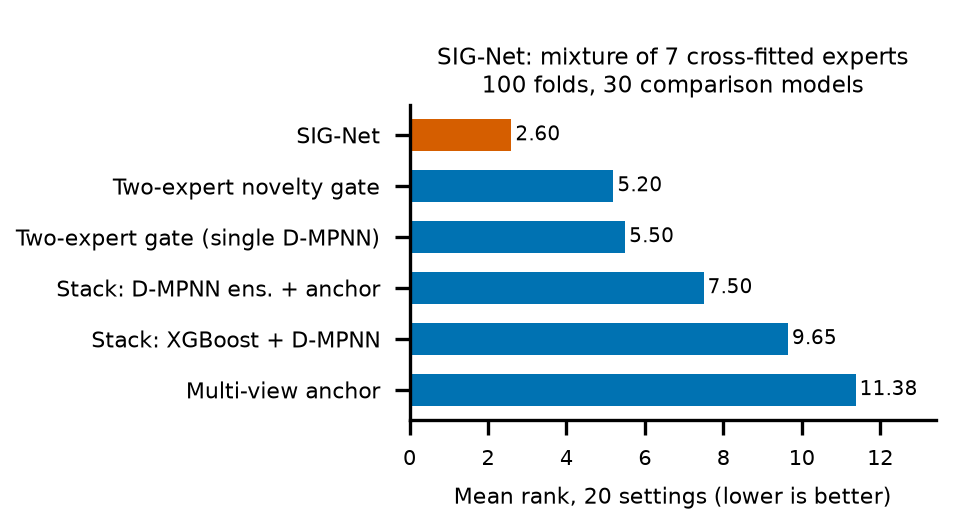
\includegraphics[width=3.25in,height=1.75in,keepaspectratio]{toc_graphic.png}
\end{tocentry}

\begin{abstract}
Molecular property models are usually validated on Bemis--Murcko (BM) scaffold splits, and no single model family wins across datasets and split protocols. We make two contributions. First, an audit of five MoleculeNet benchmarks over five seeds shows that BM scaffold splits leave 54--62\% of test molecules with a generic carbon skeleton that also occurs in the training set; generic-skeleton splits remove this overlap. Second, we introduce SIG-Net, a similarity-informed mixture of seven cross-fitted experts (four graph neural networks, two tree ensembles and a descriptor stack). Each expert is cross-fitted on the training set, and for every query molecule the experts are weighted by their out-of-fold error on its Tanimoto nearest neighbours, shrunk towards global stacking weights as structural novelty increases; all hyperparameters are selected on validation data only. Across 5 datasets $\times$ 4 split protocols $\times$ 5 seeds (100 folds) and 30 comparison models, SIG-Net has the best mean rank (2.60 vs.\ 5.20 for the next model), is best in 12/20 settings, and outperforms the strongest external stacking baseline in 80/100 folds (mean relative improvement 3.8\%, $p = 1.3 \times 10^{-9}$) and a Chemprop-style D-MPNN with RDKit features by 5.2\% (84/100 folds) and frozen ChemBERTa-2 embeddings by 23.4\% (93/100 folds). Ablations attribute most of the gain to cross-fitted stacking of diverse experts. In a pre-registered confirmation on fresh splits (57 folds), the advantage of the expert mixture over every single model replicated (5.1--28\%), the original local weighting did not ($p = 0.805$), and a refined router with a novelty-damped local out-of-fold residual correction improved on the global stack (+1.3\%, $p = 0.020$), mainly on regression endpoints. The novelty-shrinkage exponent had no measurable effect in either analysis.
\end{abstract}

\section{Introduction}
Machine-learning models of molecular properties are increasingly used to prioritise compounds whose ring systems were not seen during training. Benchmarks therefore replace random splits with grouped splits, most commonly by Bemis--Murcko (BM) scaffold\cite{bemis1996properties,wu2018moleculenet}. Several recent studies question whether such splits are as hard as assumed: Fooladi et al.\ found that scaffold splits often degrade performance only modestly relative to random splits\cite{fooladi2025evaluating}, Reimer et al.\ reported that scaffold and UMAP splits are frequently closer to random than expected\cite{reimer2025chemspace}, and Zheng et al.\ showed that holding out structurally remote scaffold groups exposes failures that scaffold splits hide\cite{zheng2026frontier}. Benchmarks such as BOOM similarly report large out-of-distribution (OOD) errors for current models\cite{boom2025}.

A second, related observation is that the best model depends on the dataset and on the split. Directed message-passing networks (D-MPNN/Chemprop)\cite{yang2019analyzing,heid2024chemprop} are strong on larger sets, while descriptor-based tree ensembles remain competitive on small ones\cite{yang2019analyzing}, and domain-invariance penalties such as Deep CORAL\cite{sun2016deep} help in some settings and not others. Stacking\cite{wolpert1992stacked} combines models with fixed weights; mixtures of experts\cite{jacobs1991adaptive} allow weights to vary per input but need enough data to learn the gating function, which small chemistry datasets rarely provide.

We address both points. (i) We audit five MoleculeNet benchmarks under four split protocols and five seeds, and quantify how often BM scaffold splits leave a test molecule's generic carbon skeleton in the training set. (ii) We propose SIG-Net, a mixture of seven cross-fitted experts in which the per-molecule weights are not learned by a gating network but estimated non-parametrically from each expert's out-of-fold error on the query's nearest training neighbours. Cross-fitting supplies an unbiased error estimate for every training molecule, so the gate is informed by the whole training set rather than by a small validation fold. We evaluate SIG-Net against 30 models, including a pretrained chemical language model, on 100 folds with a pre-specified analysis plan, and report ablations that separate the contributions of cross-fitting, expert diversity, local weighting and novelty shrinkage, including the components that do not help. Finally, we test the local components in a pre-registered confirmation on fresh splits, together with a refined router that addresses the limitations of the first.

\section{Methods}

\subsection{Datasets and curation}
We use five MoleculeNet benchmarks\cite{wu2018moleculenet}: hydration free energy (\texttt{FreeSolv}\cite{mobley2014freesolv}), aqueous solubility (\texttt{ESOL}\cite{delaney2004esol}), octanol/water distribution at pH 7.4 (\texttt{Lipophilicity}), $\beta$-secretase inhibition (\texttt{BACE}\cite{subramanian2016bace}) and blood--brain barrier penetration (\texttt{BBBP}\cite{martins2012bbbp}). Structures were standardised with RDKit\cite{rdkit} (largest-fragment selection, neutralisation, canonical isomeric SMILES) and indexed by InChIKey. Duplicates with consistent labels ($\Delta y \le 0.2\,\sigma_y$, or identical class) were merged; conflicting duplicates were removed (Table~\ref{tab:datasets}).

\subsection{Splitting protocols}
Each dataset was split 80/10/10 into training, validation and test sets under four protocols, each with five seeds (42, 100, 2026, 7, 99): \emph{random}; \emph{BM scaffold}\cite{bemis1996properties}, grouping molecules by their heavy-atom ring-and-linker framework; \emph{generic skeleton}, grouping by that framework after converting all atoms to carbon and all bonds to single bonds; and \emph{Butina cluster}\cite{butina1999unsupervised}, sphere-exclusion clustering of 2048-bit Morgan (ECFP4\cite{rogers2010extended}) fingerprints at Tanimoto distance 0.6. Grouped protocols assign groups larger than 5\% of the data to the training set and shuffle the remaining groups by seed. For each split we computed scaffold and skeleton overlap, the fraction of test molecules whose generic skeleton occurs in the training set, and the nearest-neighbour (NN) Tanimoto similarity of each test molecule to the training set.

\subsection{Featurisation}
Graph models use one-hot atom features (atomic number, degree, formal charge, chirality, hydrogen count, hybridisation, aromaticity, scaled mass; 133 dimensions) and bond features (type, conjugation, ring membership, stereochemistry; 14 dimensions) following Chemprop\cite{yang2019analyzing,heid2024chemprop}. Descriptor models use 2D RDKit descriptors clipped to the training-fold 1st--99th percentiles and standardised on the training fold, 167-bit MACCS keys\cite{durant2002reoptimization} and ECFP4 bits. All scaling, clipping and PCA statistics are fitted on the training fold only.

\subsection{Comparison models}
We evaluate random forests and XGBoost on ECFP4, MACCS, RDKit-2D and ECFP4+RDKit-2D; a gated residual MLP on ECFP4+RDKit-2D; GCN\cite{kipf2017semi}, GINE\cite{xu2019powerful}, GATv2\cite{brody2022attentive} and AttentiveFP\cite{xiong2020pushing}; D-MPNN\cite{yang2019analyzing} with and without RDKit-2D features; D-MPNN with a Deep CORAL\cite{sun2016deep} feature-alignment penalty as a domain-invariance baseline; a three-seed D-MPNN+RDKit ensemble\cite{lakshminarayanan2017simple}; two pretrained-foundation-model baselines that use frozen, mean-pooled embeddings of the chemical language model ChemBERTa-2 (77M parameters, multi-task-regression pretraining\cite{ahmad2022chemberta2}) with a ridge (logistic for classification) head whose regularisation is chosen on the validation fold, or an XGBoost head with early stopping on the validation fold; five-fold cross-fitted (bagged) versions of each SIG-Net expert; a multi-view descriptor stack (below); two stacking baselines that combine two models with a single validation-selected weight; and two earlier designs from our group, a dual-stream gated residual network and a two-expert novelty gate. Neural models use standardised regression targets, AdamW with a one-cycle learning-rate schedule for 80 epochs, and the checkpoint with the best validation score. Tree models use fixed hyperparameters; XGBoost in the baselines uses early stopping on the validation fold.

\subsection{Multi-view descriptor stack}
Five learners are fitted on the training fold---random forests on MACCS and RDKit-2D, ridge (logistic for classification) regression on all descriptor views, and XGBoost on RDKit-2D and on ECFP4+RDKit-2D (ECFP4 for classification)---and combined with non-negative weights summing to one, fitted on the validation fold. Out-of-fold training-set predictions of this stack are obtained by three-fold scaffold-grouped cross-fitting.

\subsection{SIG-Net}
\paragraph{Experts and cross-fitting.} SIG-Net combines $M = 7$ experts: D-MPNN+RDKit, D-MPNN+RDKit with Deep CORAL, GINE, AttentiveFP, XGBoost on ECFP4+RDKit-2D, a random forest on RDKit-2D, and the multi-view descriptor stack. The training set is divided into $K = 5$ scaffold-grouped folds. Each expert $m$ is trained $K$ times, each time on $K-1$ folds, which gives an out-of-fold prediction $o_m(j)$ for every training molecule $j$. Validation and test predictions $p_m(x)$ are the means of the $K$ models.

\paragraph{Global weights.} Non-negative weights $\mathbf{w}^{\mathrm{glob}}$ summing to one are fitted by minimising the squared error of $\sum_m w_m o_m(j)$ on all training molecules (Brier score for classification).

\paragraph{Local competence.} For a query molecule $x$ let $\mathcal{N}_k(x)$ be its $k$ most similar training molecules (ECFP4 Tanimoto similarity $s_j$). The local error of expert $m$ is
\begin{equation}
e_m(x) = \frac{\sum_{j \in \mathcal{N}_k(x)} s_j\,\bigl(y_j - o_m(j)\bigr)^2}{\sum_{j \in \mathcal{N}_k(x)} s_j},
\end{equation}
with targets standardised for regression, and the local weights are $w^{\mathrm{loc}}_m(x) \propto \exp\!\bigl(-e_m(x) / (\tau\,\tilde{e}(x))\bigr)$, where $\tilde{e}(x)$ is the median of $e_m(x)$ over experts.

\paragraph{Novelty shrinkage.} The final weights interpolate between local and global weights according to the mean neighbour similarity $\bar{s}_k(x)$:
\begin{equation}
\mathbf{w}(x) = \lambda(x)\,\mathbf{w}^{\mathrm{loc}}(x) + \bigl(1 - \lambda(x)\bigr)\,\mathbf{w}^{\mathrm{glob}}, \qquad \lambda(x) = \bar{s}_k(x)^{\gamma},
\end{equation}
and the prediction is $\hat{y}(x) = \sum_m w_m(x)\,p_m(x)$.

\paragraph{Model selection.} The neighbourhood size $k \in \{5, 10, 20, 50\}$, temperature $\tau \in \{0.25, 0.5, 1, 2\}$ and shrinkage exponent $\gamma \in \{0, 1, 2, 4\}$, together with the purely global combination, are selected per fold by the validation score. The test fold is not used for any fitting or selection step. The overall design (expert set, $K$ and the grids) was fixed using validation scores on three development folds before the final run.

\subsection{Refined router (SIG-Net v4) and confirmatory design}
To address the limitations of the softmax router we developed a second router, evaluated only on fresh splits. Let $r_j \in \mathbb{R}^M$ be the standardised out-of-fold residuals of the $M$ experts on training molecule $j$, and $\boldsymbol{\Sigma}_{\mathrm{glob}} = N^{-1}\sum_j r_j r_j^\top$. For a query $x$, neighbours are taken under a composite kernel $K(x,j) = a\,s_{\mathrm{ECFP}} + (1-a)\,(s_{\mathrm{MACCS}} + s_{\mathrm{phys}})/2$, where $s_{\mathrm{phys}}$ is an RBF kernel on standardised RDKit descriptors (median-distance bandwidth). With neighbour weights $\omega_j \propto K(x,j)^2$ over the $k$ nearest training molecules,
\begin{equation}
\hat{\boldsymbol{\Sigma}}(x) = \lambda(x)\sum_{j \in \mathcal{N}_k(x)} \omega_j r_j r_j^\top + \bigl(1-\lambda(x)\bigr)\boldsymbol{\Sigma}_{\mathrm{glob}}, \qquad \lambda(x) = \bar{s}_k(x)^{\gamma},
\end{equation}
\begin{equation}
\begin{aligned}
\mathbf{w}(x) &= \arg\min_{\mathbf{w} \in \Delta^{M-1}} \mathbf{w}^\top \bigl(\hat{\boldsymbol{\Sigma}}(x) + \rho\,\mathrm{tr}(\hat{\boldsymbol{\Sigma}}(x))\,\mathbf{I}/M\bigr)\,\mathbf{w}, \\
\hat{y}(x) &= \mathbf{w}(x)^\top \mathbf{p}(x) + \nu\,\bar{s}_k(x)^{\gamma_d} \sum_{j \in \mathcal{N}_k(x)} \omega_j \bigl(y_j - \mathbf{w}(x)^\top \mathbf{o}(j)\bigr),
\end{aligned}
\end{equation}
where $\bar{s}_k(x)$ is the mean ECFP similarity of the neighbours and $\mathbf{o}(j)$ the out-of-fold expert predictions. For squared loss the global stack solves the same problem with $\boldsymbol{\Sigma}_{\mathrm{glob}}$, so it is the special case $\lambda = 0$, $\nu = 0$. The weights are computed by projected gradient descent on the simplex; $k \in \{10, 25, 50\}$, $a \in \{0.5, 0.75, 1\}$, $\gamma \in \{0, 0.5, 1, 2, 4\}$ (or the global weights), $\nu \in \{0, 0.25, 0.5, 0.75\}$ and $\gamma_d \in \{1, 2\}$ are selected per fold on the validation set, with $\rho = 0.05$.

The confirmation used new split seeds (development seed 11; confirmatory seeds 1--3) produced by the same splitting code, and nine cross-fitted experts (the seven SIG-Net experts, ChemBERTa-2 + XGBoost and XGBoost on ECFP4) whose out-of-fold, validation and test predictions were stored. The v4 variant (7 or 9 experts, with or without each component) was chosen on the development seed by a rule fixed beforehand; the design was then frozen (file hashes recorded) before any confirmatory result was computed. The primary endpoint---SIG-Net v4 vs.\ the global stack of the seven original experts over all confirmatory folds except the degenerate \texttt{FreeSolv} generic-skeleton split---and the secondary comparisons were registered in advance (Supporting Information).

\subsection{Evaluation and statistics}
Regression tasks are scored by test RMSE and the classification tasks (\texttt{BACE}, \texttt{BBBP}) by ROC-AUC. Each of the 20 dataset--protocol settings is run with five seeds (100 folds per model). We report mean $\pm$ SD over seeds; mean ranks across the 20 settings with a Friedman test and Nemenyi critical difference\cite{demsar2006statistical}; and paired comparisons over all 100 folds using the two-sided Wilcoxon signed-rank test on the per-fold relative improvement. The primary comparison and all secondary analyses were specified in an analysis plan written before the final test results were viewed; \texttt{BBBP} and the ChemBERTa-2 baselines were added later, under a written addendum made before their results were viewed (Supporting Information). Per-setting paired $t$-tests over five seeds are reported as descriptive statistics.


\begin{table}
\caption{Curated datasets.}
\label{tab:datasets}
\small
\begin{tabular}{llcccc}
\toprule
Dataset & Task (unit) & Raw $\to$ curated & BM scaffolds & Generic skeletons & Singleton BM \\
\midrule
\texttt{FreeSolv} & Regression (kcal/mol) & 642 $\to$ 642 & 63 & 32 & 57.1\% \\
\texttt{ESOL} & Regression (log mol/L) & 1128 $\to$ 1116 & 269 & 167 & 73.2\% \\
\texttt{Lipophilicity} & Regression ($\log D_{7.4}$) & 4200 $\to$ 4200 & 2408 & 1516 & 77.1\% \\
\texttt{BACE} & Classification (binary) & 1513 $\to$ 1509 & 648 & 376 & 69.6\% \\
\texttt{BBBP} & Classification (binary) & 2039 $\to$ 1950 & 1012 & 686 & 76.1\% \\
\bottomrule
\end{tabular}
\end{table}

\section{Results}

\subsection{BM scaffold splits leave most test molecules with a seen carbon skeleton}
\begin{table*}
\caption{Split diagnostics, mean $\pm$ SD over five seeds. Overlaps are percentages of unique test scaffolds; ``Seen skeleton'' is the percentage of test molecules whose generic skeleton occurs in training; ``Hard OOD'': test molecules with NN Tanimoto $< 0.45$. $^{a}$All five seeds give the same test set.}
\label{tab:splits}
\scriptsize
\begin{tabular}{llccccc}
\toprule
Dataset & Split & BM overlap (\%) & Skeleton overlap (\%) & Seen skeleton (\% mols) & NN Tanimoto & Hard OOD (\%) \\
\midrule
\texttt{FreeSolv} & Random & 66.6 $\pm$ 11.7 & 80.8 $\pm$ 10.9 & 96.9 $\pm$ 1.9 & 0.559 $\pm$ 0.023 & 28.8 $\pm$ 6.6 \\
 & BM scaffold & 0.0 $\pm$ 0.0 & 39.3 $\pm$ 6.2 & 62.5 $\pm$ 15.1 & 0.381 $\pm$ 0.043 & 67.5 $\pm$ 11.2 \\
 & Generic skeleton$^{a}$ & 0.0 $\pm$ 0.0 & 0.0 $\pm$ 0.0 & 0.0 $\pm$ 0.0 & 0.372 $\pm$ 0.000 & 81.6 $\pm$ 0.0 \\
 & Butina cluster & 60.6 $\pm$ 14.4 & 88.6 $\pm$ 10.6 & 96.9 $\pm$ 3.3 & 0.439 $\pm$ 0.037 & 56.9 $\pm$ 14.0 \\
\midrule
\texttt{ESOL} & Random & 51.1 $\pm$ 5.6 & 62.8 $\pm$ 8.3 & 88.1 $\pm$ 2.2 & 0.559 $\pm$ 0.013 & 29.7 $\pm$ 2.0 \\
 & BM scaffold & 0.0 $\pm$ 0.0 & 36.7 $\pm$ 4.1 & 60.5 $\pm$ 4.5 & 0.435 $\pm$ 0.044 & 56.8 $\pm$ 10.3 \\
 & Generic skeleton & 0.0 $\pm$ 0.0 & 0.0 $\pm$ 0.0 & 0.0 $\pm$ 0.0 & 0.430 $\pm$ 0.025 & 59.5 $\pm$ 8.5 \\
 & Butina cluster & 42.9 $\pm$ 4.4 & 60.8 $\pm$ 11.5 & 89.4 $\pm$ 4.9 & 0.446 $\pm$ 0.015 & 54.1 $\pm$ 4.6 \\
\midrule
\texttt{Lipophilicity} & Random & 44.5 $\pm$ 3.2 & 62.0 $\pm$ 4.4 & 72.1 $\pm$ 3.0 & 0.646 $\pm$ 0.009 & 22.6 $\pm$ 1.7 \\
 & BM scaffold & 0.0 $\pm$ 0.0 & 41.2 $\pm$ 1.3 & 54.4 $\pm$ 5.5 & 0.560 $\pm$ 0.014 & 32.6 $\pm$ 4.0 \\
 & Generic skeleton & 0.0 $\pm$ 0.0 & 0.0 $\pm$ 0.0 & 0.0 $\pm$ 0.0 & 0.538 $\pm$ 0.016 & 34.9 $\pm$ 4.1 \\
 & Butina cluster & 14.2 $\pm$ 1.7 & 34.1 $\pm$ 1.6 & 41.0 $\pm$ 5.5 & 0.397 $\pm$ 0.031 & 76.4 $\pm$ 7.8 \\
\midrule
\texttt{BACE} & Random & 57.9 $\pm$ 2.7 & 73.3 $\pm$ 4.8 & 82.6 $\pm$ 3.6 & 0.797 $\pm$ 0.009 & 1.9 $\pm$ 0.3 \\
 & BM scaffold & 0.0 $\pm$ 0.0 & 51.1 $\pm$ 4.9 & 60.4 $\pm$ 7.1 & 0.723 $\pm$ 0.009 & 5.0 $\pm$ 1.5 \\
 & Generic skeleton & 0.0 $\pm$ 0.0 & 0.0 $\pm$ 0.0 & 0.0 $\pm$ 0.0 & 0.692 $\pm$ 0.045 & 6.8 $\pm$ 8.1 \\
 & Butina cluster & 8.7 $\pm$ 2.3 & 22.3 $\pm$ 6.4 & 31.9 $\pm$ 7.6 & 0.539 $\pm$ 0.046 & 36.0 $\pm$ 10.3 \\
\midrule
\texttt{BBBP} & Random & 42.9 $\pm$ 3.0 & 58.7 $\pm$ 2.8 & 74.5 $\pm$ 2.0 & 0.565 $\pm$ 0.013 & 32.1 $\pm$ 3.2 \\
 & BM scaffold & 0.0 $\pm$ 0.0 & 40.4 $\pm$ 2.5 & 61.1 $\pm$ 9.9 & 0.497 $\pm$ 0.021 & 38.5 $\pm$ 8.5 \\
 & Generic skeleton & 0.0 $\pm$ 0.0 & 0.0 $\pm$ 0.0 & 0.0 $\pm$ 0.0 & 0.464 $\pm$ 0.020 & 49.4 $\pm$ 5.9 \\
 & Butina cluster & 19.6 $\pm$ 3.1 & 38.8 $\pm$ 3.3 & 57.6 $\pm$ 6.1 & 0.381 $\pm$ 0.023 & 78.1 $\pm$ 6.3 \\
\bottomrule
\end{tabular}
\end{table*}

Table~\ref{tab:splits} and Figure~\ref{fig:leakage} summarise the split audit. BM scaffold splits have no shared BM scaffolds by construction, but 37--51\% of test scaffolds reduce to a generic skeleton that also occurs in training, and 54--62\% of test \emph{molecules} have such a skeleton. Generic-skeleton splits remove this overlap entirely and lower the mean nearest-neighbour (NN) similarity on \texttt{FreeSolv}, \texttt{ESOL} and \texttt{Lipophilicity}. Butina clustering at a Tanimoto distance of 0.6 behaves differently by dataset: on the small, chemically simple \texttt{FreeSolv} and \texttt{ESOL} sets it leaves 89--97\% of test molecules with a seen generic skeleton, whereas on \texttt{Lipophilicity}, \texttt{BACE} and \texttt{BBBP} it produces the most novel test sets (NN similarity 0.40, 0.54, 0.38). On \texttt{FreeSolv}, the generic-skeleton protocol yields the same test set for all five seeds because a few large skeleton groups dominate the dataset; results for that setting reflect model variance only and are flagged throughout.

\begin{figure}
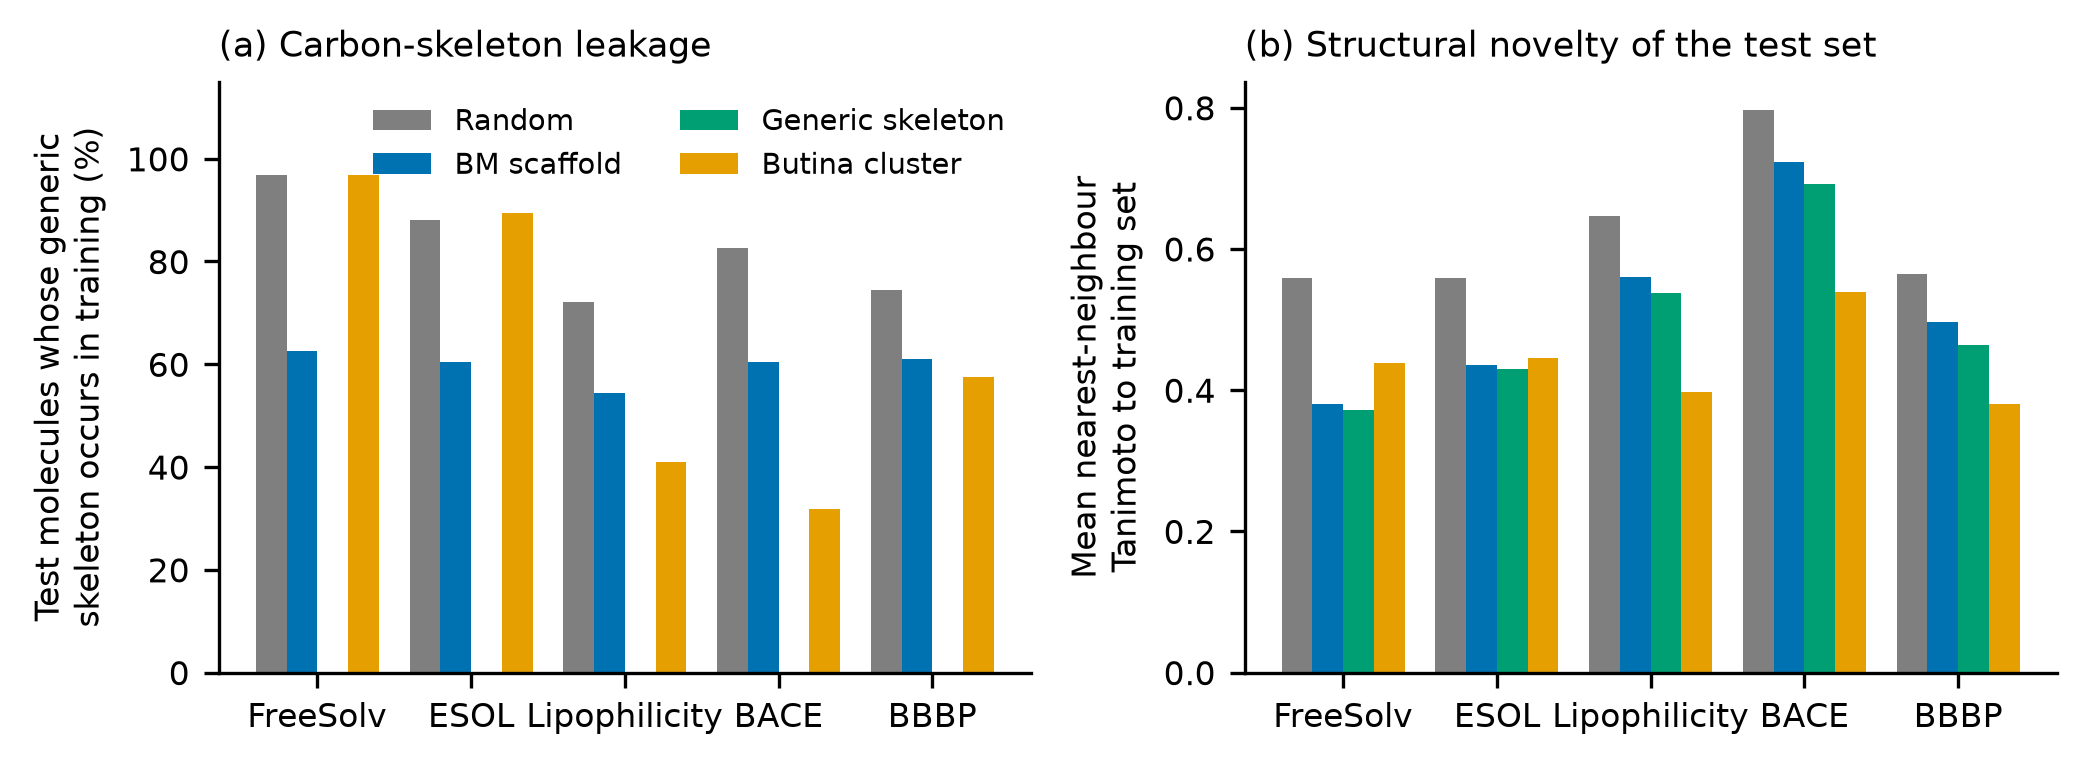
\includegraphics[width=\textwidth]{fig1_leakage.png}
\caption{Split audit over five seeds. (a) Percentage of test molecules whose generic carbon skeleton occurs in the training set. (b) Mean nearest-neighbour ECFP4 Tanimoto similarity of test molecules to the training set.}
\label{fig:leakage}
\end{figure}

\subsection{SIG-Net has the best average rank across datasets and splits}
Table~\ref{tab:main} lists test performance for representative models; all 33 models are reported in Table~S1. Graph models trained with one-hot features reach accuracies in line with published Chemprop results (e.g.\ \texttt{Lipophilicity} random split RMSE 0.54 for D-MPNN+RDKit). Ranking the 31 models that are not internal ablations of SIG-Net within each of the 20 settings (Figure~\ref{fig:ranks}, Table~S2), SIG-Net has a mean rank of 2.60 (2.87 on the 15 OOD settings) against 5.20 for the next model (Two-expert novelty gate). It is first in 12 of 20 settings: 2 of four \texttt{FreeSolv}, 3 of four \texttt{ESOL}, 4 of four \texttt{Lipophilicity}, 1 of four \texttt{BACE} and 2 of four \texttt{BBBP}. The Friedman test rejects equal ranks ($\chi^2 = 282$, $p = 8.0 \times 10^{-43}$); with 31 models and 20 settings the Nemenyi critical difference is 10.2 ranks, so this conservative post-hoc test separates SIG-Net only from models with mean rank above 12.8. We therefore also report paired fold-level comparisons.

\begin{table*}
\caption{Test performance (mean $\pm$ SD over five seeds). RMSE for regression (lower is better), ROC-AUC for \texttt{BACE} and \texttt{BBBP} (higher is better). Bold: best among the columns shown. All models are reported in Table~S1.}
\label{tab:main}
\scriptsize
\resizebox{\textwidth}{!}{%
\begin{tabular}{llcccccccc}
\toprule
Dataset & Split & \makecell{XGBoost\\ECFP4+RDKit} & \makecell{AttentiveFP} & \makecell{D-MPNN} & \makecell{D-MPNN\\+RDKit} & \makecell{D-MPNN+RDKit\\5-fold bagged} & \makecell{Stack\\XGB+D-MPNN} & \makecell{Global stack\\(same experts)} & \makecell{\textbf{SIG-Net}} \\
\midrule
\texttt{FreeSolv} & Random & 1.066 $\pm$ 0.404 & 0.983 $\pm$ 0.085 & 1.111 $\pm$ 0.066 & 0.871 $\pm$ 0.135 & 0.870 $\pm$ 0.258 & 0.884 $\pm$ 0.146 & 0.822 $\pm$ 0.229 & \textbf{0.800 $\pm$ 0.211} \\
 & BM scaffold & 2.464 $\pm$ 0.478 & 2.030 $\pm$ 0.544 & 1.823 $\pm$ 0.097 & 1.723 $\pm$ 0.197 & 1.795 $\pm$ 0.094 & 1.880 $\pm$ 0.292 & 1.719 $\pm$ 0.131 & 1.720 $\pm$ 0.136 \\
 & Generic skeleton & 1.773 $\pm$ 0.072 & 1.363 $\pm$ 0.129 & \textbf{1.337 $\pm$ 0.066} & 1.525 $\pm$ 0.065 & 1.556 $\pm$ 0.027 & 1.474 $\pm$ 0.074 & 1.465 $\pm$ 0.055 & 1.405 $\pm$ 0.054 \\
 & Butina cluster & 1.157 $\pm$ 0.350 & 1.097 $\pm$ 0.164 & 1.219 $\pm$ 0.250 & 1.089 $\pm$ 0.118 & 1.115 $\pm$ 0.207 & 1.057 $\pm$ 0.133 & 1.081 $\pm$ 0.225 & \textbf{1.038 $\pm$ 0.155} \\
\midrule
\texttt{ESOL} & Random & 0.597 $\pm$ 0.013 & 0.570 $\pm$ 0.059 & 0.652 $\pm$ 0.080 & 0.557 $\pm$ 0.025 & 0.536 $\pm$ 0.035 & 0.532 $\pm$ 0.024 & 0.516 $\pm$ 0.039 & \textbf{0.511 $\pm$ 0.042} \\
 & BM scaffold & 0.788 $\pm$ 0.105 & 0.849 $\pm$ 0.123 & 0.861 $\pm$ 0.061 & 0.777 $\pm$ 0.065 & 0.762 $\pm$ 0.086 & \textbf{0.751 $\pm$ 0.065} & 0.763 $\pm$ 0.108 & 0.754 $\pm$ 0.112 \\
 & Generic skeleton & 0.787 $\pm$ 0.097 & 0.807 $\pm$ 0.089 & 0.890 $\pm$ 0.168 & 0.736 $\pm$ 0.083 & 0.730 $\pm$ 0.079 & 0.717 $\pm$ 0.096 & \textbf{0.696 $\pm$ 0.097} & 0.704 $\pm$ 0.093 \\
 & Butina cluster & 0.594 $\pm$ 0.124 & 0.602 $\pm$ 0.059 & 0.641 $\pm$ 0.113 & 0.568 $\pm$ 0.087 & 0.565 $\pm$ 0.084 & 0.563 $\pm$ 0.092 & \textbf{0.544 $\pm$ 0.082} & 0.544 $\pm$ 0.080 \\
\midrule
\texttt{Lipophilicity} & Random & 0.597 $\pm$ 0.045 & 0.545 $\pm$ 0.041 & 0.527 $\pm$ 0.044 & 0.544 $\pm$ 0.036 & 0.542 $\pm$ 0.034 & 0.531 $\pm$ 0.043 & 0.506 $\pm$ 0.047 & \textbf{0.505 $\pm$ 0.047} \\
 & BM scaffold & 0.693 $\pm$ 0.028 & 0.614 $\pm$ 0.032 & 0.646 $\pm$ 0.096 & 0.665 $\pm$ 0.033 & 0.648 $\pm$ 0.033 & 0.637 $\pm$ 0.030 & \textbf{0.576 $\pm$ 0.038} & 0.580 $\pm$ 0.037 \\
 & Generic skeleton & 0.698 $\pm$ 0.051 & 0.634 $\pm$ 0.042 & 0.636 $\pm$ 0.040 & 0.670 $\pm$ 0.041 & 0.649 $\pm$ 0.047 & 0.636 $\pm$ 0.046 & 0.590 $\pm$ 0.033 & \textbf{0.589 $\pm$ 0.033} \\
 & Butina cluster & 0.809 $\pm$ 0.053 & 0.724 $\pm$ 0.042 & 0.717 $\pm$ 0.074 & 0.764 $\pm$ 0.061 & 0.744 $\pm$ 0.065 & 0.735 $\pm$ 0.058 & 0.670 $\pm$ 0.044 & \textbf{0.668 $\pm$ 0.041} \\
\midrule
\texttt{BACE} & Random & 0.889 $\pm$ 0.030 & 0.872 $\pm$ 0.031 & 0.887 $\pm$ 0.024 & 0.879 $\pm$ 0.037 & 0.883 $\pm$ 0.035 & 0.892 $\pm$ 0.032 & \textbf{0.901 $\pm$ 0.022} & 0.900 $\pm$ 0.021 \\
 & BM scaffold & 0.849 $\pm$ 0.044 & 0.836 $\pm$ 0.040 & 0.840 $\pm$ 0.044 & 0.830 $\pm$ 0.068 & 0.840 $\pm$ 0.065 & 0.841 $\pm$ 0.067 & 0.863 $\pm$ 0.045 & \textbf{0.864 $\pm$ 0.046} \\
 & Generic skeleton & 0.789 $\pm$ 0.079 & 0.806 $\pm$ 0.065 & 0.731 $\pm$ 0.102 & 0.812 $\pm$ 0.086 & 0.816 $\pm$ 0.082 & 0.807 $\pm$ 0.077 & 0.810 $\pm$ 0.079 & 0.815 $\pm$ 0.081 \\
 & Butina cluster & 0.759 $\pm$ 0.091 & 0.704 $\pm$ 0.099 & 0.745 $\pm$ 0.080 & 0.781 $\pm$ 0.043 & 0.782 $\pm$ 0.049 & 0.762 $\pm$ 0.066 & 0.767 $\pm$ 0.114 & 0.790 $\pm$ 0.076 \\
\midrule
\texttt{BBBP} & Random & 0.926 $\pm$ 0.015 & 0.892 $\pm$ 0.062 & 0.906 $\pm$ 0.022 & 0.926 $\pm$ 0.017 & 0.926 $\pm$ 0.011 & 0.931 $\pm$ 0.012 & 0.935 $\pm$ 0.010 & \textbf{0.940 $\pm$ 0.007} \\
 & BM scaffold & 0.933 $\pm$ 0.030 & 0.898 $\pm$ 0.031 & 0.929 $\pm$ 0.017 & 0.916 $\pm$ 0.050 & 0.914 $\pm$ 0.052 & 0.935 $\pm$ 0.024 & 0.939 $\pm$ 0.033 & \textbf{0.940 $\pm$ 0.029} \\
 & Generic skeleton & 0.949 $\pm$ 0.019 & 0.923 $\pm$ 0.046 & 0.912 $\pm$ 0.075 & 0.927 $\pm$ 0.038 & 0.934 $\pm$ 0.030 & 0.936 $\pm$ 0.035 & 0.952 $\pm$ 0.023 & \textbf{0.954 $\pm$ 0.025} \\
 & Butina cluster & 0.855 $\pm$ 0.046 & 0.818 $\pm$ 0.060 & 0.821 $\pm$ 0.040 & 0.856 $\pm$ 0.040 & 0.848 $\pm$ 0.054 & 0.856 $\pm$ 0.038 & 0.881 $\pm$ 0.032 & \textbf{0.887 $\pm$ 0.033} \\
\bottomrule
\end{tabular}}
\end{table*}

\begin{figure}
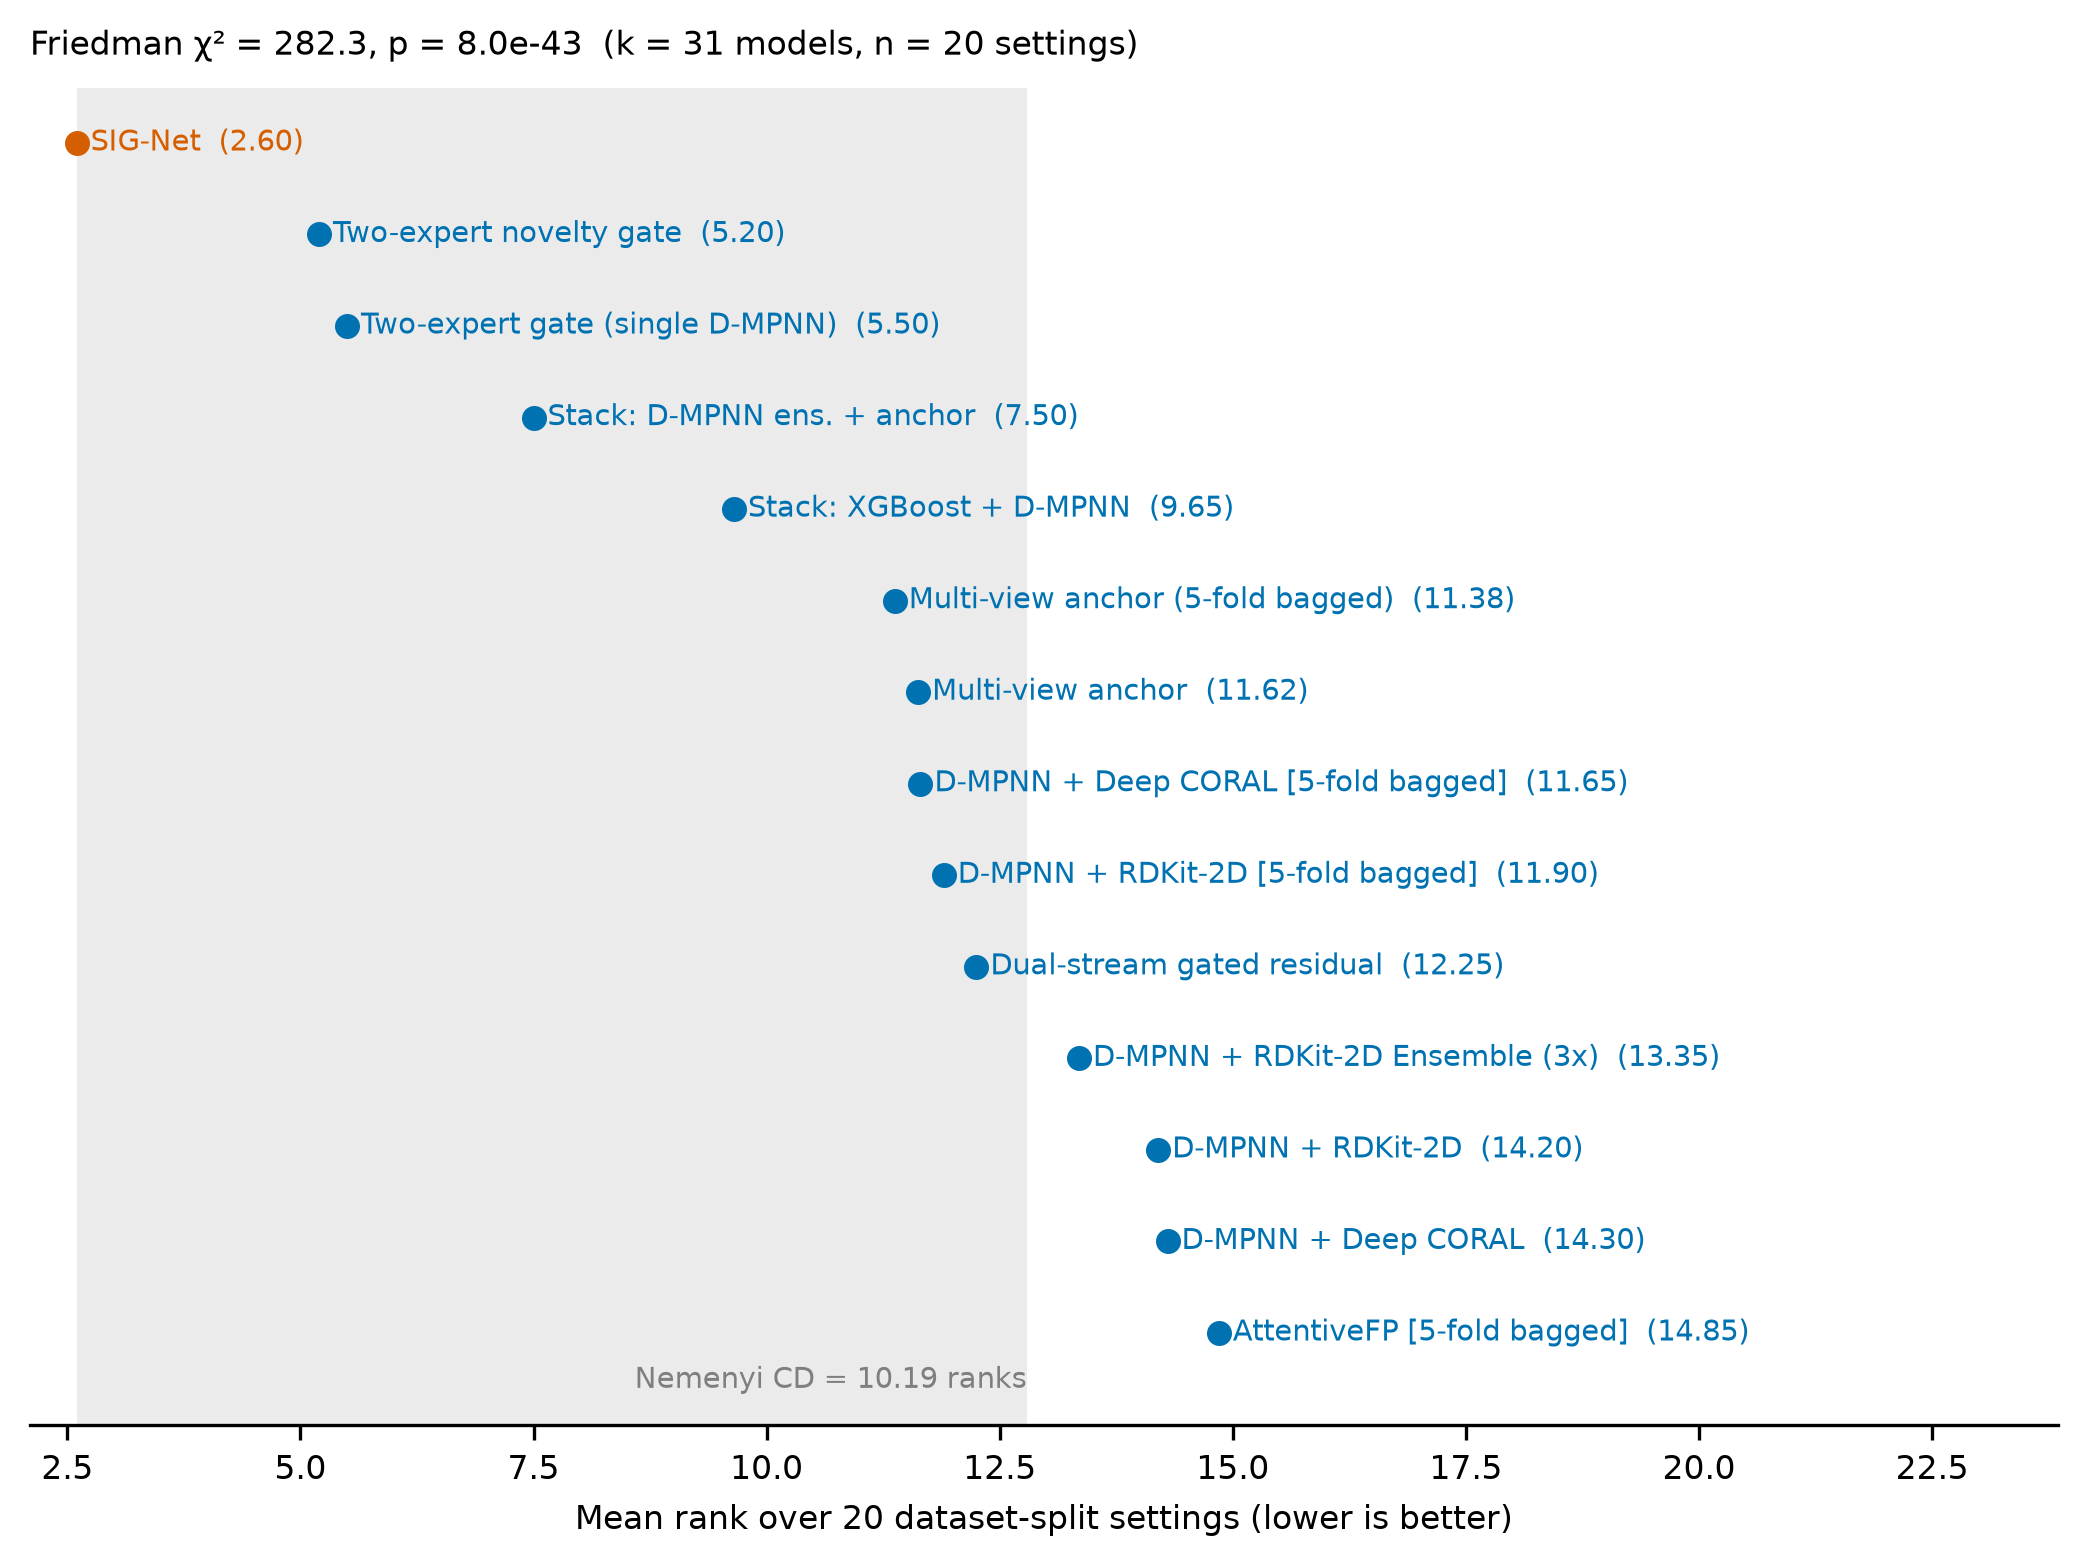
\includegraphics[width=\columnwidth]{fig2_ranks.png}
\caption{Mean rank over 20 dataset--split settings (top 14 of 31 models; internal SIG-Net ablations excluded). The grey band spans one Nemenyi critical difference from the best model.}
\label{fig:ranks}
\end{figure}

\subsection{Paired comparisons over 100 folds}
Table~\ref{tab:h2h} compares SIG-Net with selected models on every fold. SIG-Net outperforms every external model in at least 68 of 100 folds, with all two-sided Wilcoxon $p$-values at or below $1.6 \times 10^{-5}$. Against the strongest external stacking baseline (XGBoost + D-MPNN with a validation-selected weight) the mean relative improvement is 3.8\% (better in 19/20 settings); against D-MPNN+RDKit it is 5.2\% and against our earlier two-expert novelty gate 2.7\%. The frozen ChemBERTa-2 baselines are much weaker on the regression tasks: overall, SIG-Net improves on the linear probe by 20.8\% and on the XGBoost head by 23.4\% (93/100 folds). On the classification tasks, however, the ChemBERTa-2 + XGBoost baseline is competitive and has the best mean in 2 settings (\texttt{BACE} butina cluster, \texttt{BACE} generic skeleton), which suggests that pretrained representations are a promising additional expert for classification endpoints. The pre-specified primary comparison was against the strongest non-SIG-Net model by mean rank, which turned out to be the global stack of the same cross-fitted experts. On the 80 pre-specified folds (four original datasets) SIG-Net improves on it in 46/80 folds and 11/16 settings (mean +0.92\%, median +0.06\%, $p = 0.014$); including \texttt{BBBP} the figures are 60/100 folds and 15/20 settings (mean +0.80\%, $p = 0.0035$). This effect is small and, as shown below, it did not replicate on fresh splits.

\begin{table}
\caption{Paired comparison of SIG-Net with selected models over 100 folds. Relative improvement is computed per fold (RMSE reduction or AUC increase, \%); $p$: two-sided Wilcoxon signed-rank test. Full list in Table~S3.}
\label{tab:h2h}
\scriptsize
\begin{tabular}{lccrrc}
\toprule
Comparator & Folds won & Settings won & Mean (\%) & Median (\%) & $p$ \\
\midrule
Global stack (same experts) & 60/100 & 15/20 & +0.80 & +0.14 & $p = 0.0035$ \\
SIG-Net w/o novelty shrinkage & 27/100 & 9/20 & +0.05 & +0.00 & $p = 0.166$ \\
Two-expert novelty gate & 69/100 & 15/20 & +2.67 & +1.47 & $p = 8.2 \times 10^{-6}$ \\
Stack: XGBoost + D-MPNN & 80/100 & 19/20 & +3.85 & +2.75 & $p = 1.3 \times 10^{-9}$ \\
Stack: D-MPNN ens. + anchor & 73/100 & 19/20 & +3.18 & +1.89 & $p = 2.0 \times 10^{-7}$ \\
D-MPNN + RDKit-2D [5-fold bagged] & 88/100 & 19/20 & +4.72 & +4.38 & $p = 1.6 \times 10^{-13}$ \\
D-MPNN + RDKit-2D & 84/100 & 19/20 & +5.23 & +4.72 & $p = 2.4 \times 10^{-11}$ \\
D-MPNN + Deep CORAL & 82/100 & 19/20 & +5.18 & +4.64 & $p = 3.8 \times 10^{-11}$ \\
AttentiveFP & 87/100 & 19/20 & +7.41 & +6.32 & $p = 1.7 \times 10^{-13}$ \\
Multi-view anchor & 76/100 & 18/20 & +5.70 & +2.48 & $p = 6.2 \times 10^{-10}$ \\
D-MPNN (Chemprop) & 89/100 & 19/20 & +8.96 & +6.42 & $p = 8.7 \times 10^{-15}$ \\
XGBoost (ECFP4 + RDKit-2D) & 90/100 & 20/20 & +9.75 & +7.36 & $p = 1.7 \times 10^{-14}$ \\
\bottomrule
\end{tabular}
\end{table}

\subsection{Where the improvement comes from}
Table~\ref{tab:ablation} decomposes the improvement over a single D-MPNN+RDKit model. Ensembling D-MPNNs alone, either over seeds or by cross-fitting, changes little (+0.4\% and +0.5\%). Combining heterogeneous experts accounts for most of the gain: a global stack of the seven cross-fitted experts improves by +4.5\%, compared with +2.6\% for the two-expert gate. Local competence weighting adds a further +0.7 points. Shrinking local weights towards global weights as a function of novelty does not help further: SIG-Net and its variant without shrinkage are indistinguishable (27/100 folds, $p = 0.166$), and validation-based selection chose no shrinkage ($\gamma = 0$) in 56 of 100 folds and the purely global combination in 6. The simpler variant without shrinkage is therefore an equally valid choice.

\begin{table}
\caption{Ablation: mean per-fold relative improvement over a single D-MPNN+RDKit model (100 folds; RMSE reduction or AUC increase, \%).}
\label{tab:ablation}
\small
\begin{tabular}{lr}
\toprule
Model & Improvement (\%) \\
\midrule
Single D-MPNN+RDKit (reference) & +0.00 \\
D-MPNN+RDKit, 3-seed ensemble & +0.38 \\
D-MPNN+RDKit, 5-fold cross-fitted bag & +0.52 \\
Two-expert novelty gate (D-MPNN ens.\ + anchor) & +2.63 \\
Global stack of 7 cross-fitted experts & +4.46 \\
+ local competence weighting (no shrinkage) & +5.13 \\
+ novelty shrinkage = \textbf{SIG-Net} & +5.23 \\
\bottomrule
\end{tabular}
\end{table}

\subsection{Behaviour as a function of structural novelty}
Figure~\ref{fig:novelty} stratifies absolute errors on the OOD folds of the three regression datasets by the NN similarity of each test molecule. Errors grow with novelty for every model. SIG-Net reduces the error of the XGBoost + D-MPNN stack by a similar margin in every bin (7.6\%, 6.9\%, 8.2\% for NN similarity 0.00--0.35, 0.35--0.50, 0.50--1.00). The additional benefit of local weighting over the global stack is confined to the novel bins (+0.39\%, +0.50\%, -0.08\%), consistent with neighbourhood-specific expert reliability mattering most away from the training distribution, although the effect is small. Figure~\ref{fig:weights} shows the learned weights: they differ far more between datasets than between novelty bins. On \texttt{Lipophilicity} SIG-Net relies mainly on graph experts (AttentiveFP and GINE together receive 51\% of the weight), whereas on the classification sets the largest weights go to the descriptor stack, XGBoost, random forest (\texttt{BACE}); XGBoost, the descriptor stack, D-MPNN (\texttt{BBBP}). This dataset dependence is the main reason a fixed choice of model is suboptimal across benchmarks.

\begin{figure}
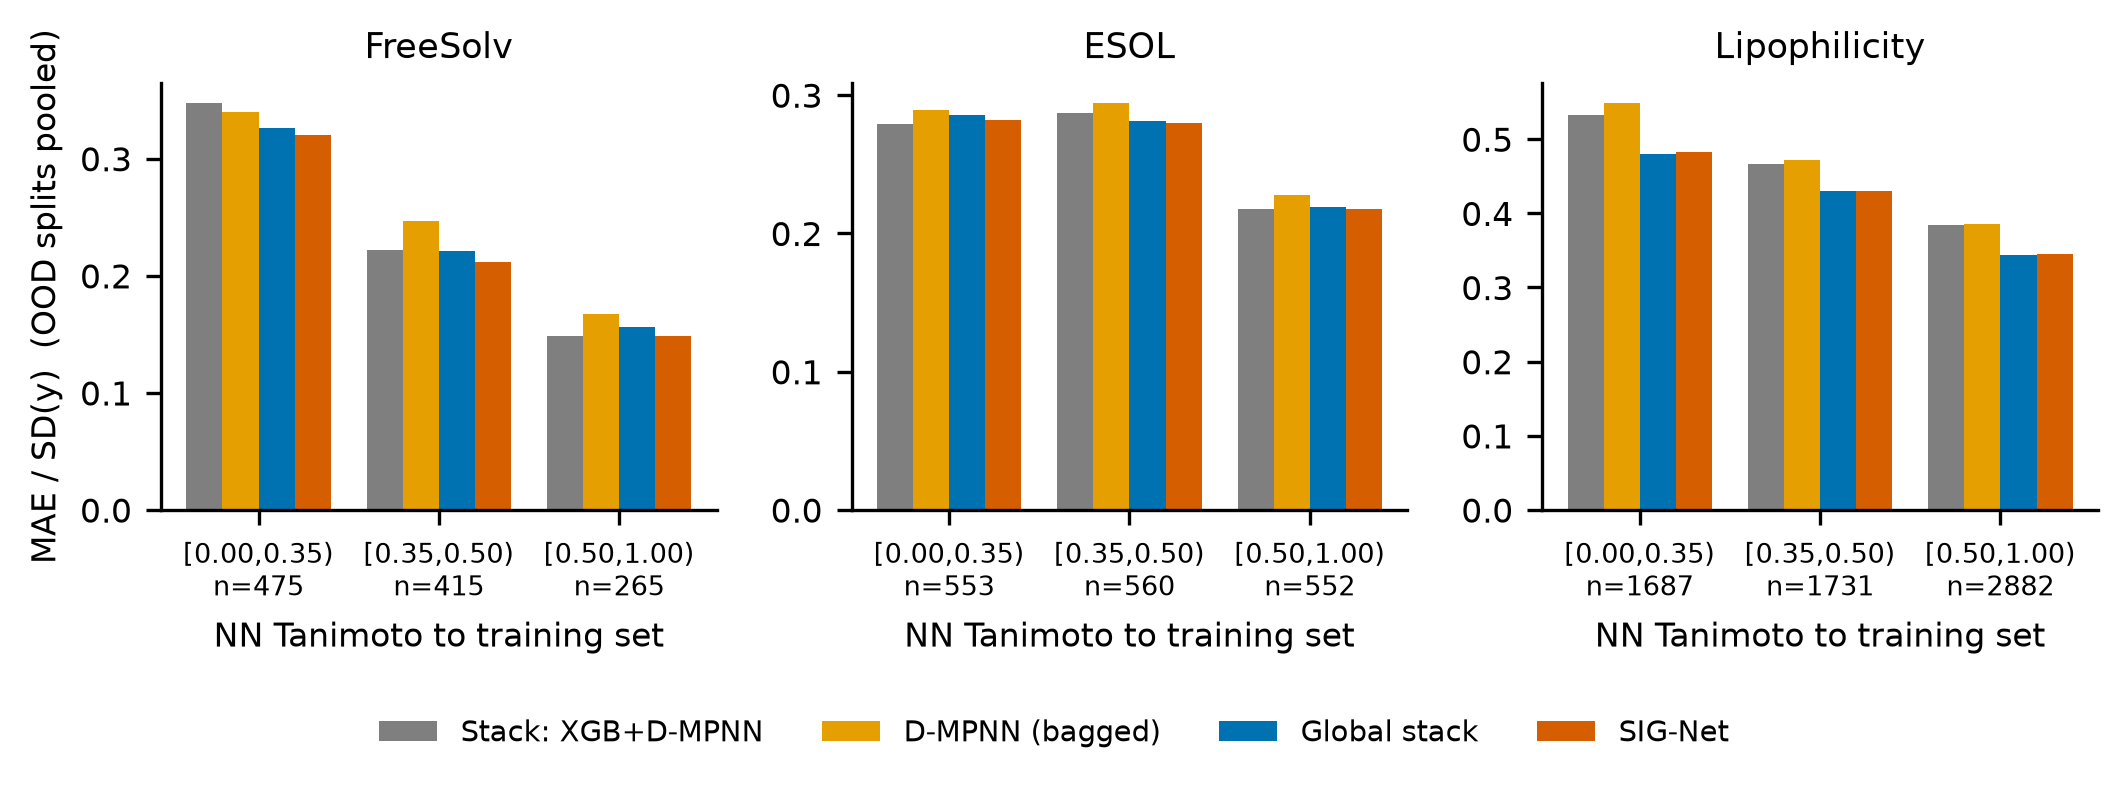
\includegraphics[width=\textwidth]{fig3_novelty.png}
\caption{Mean absolute error (normalised by the target SD) on OOD folds, stratified by the nearest-neighbour Tanimoto similarity of each test molecule to its training set.}
\label{fig:novelty}
\end{figure}

\begin{figure}
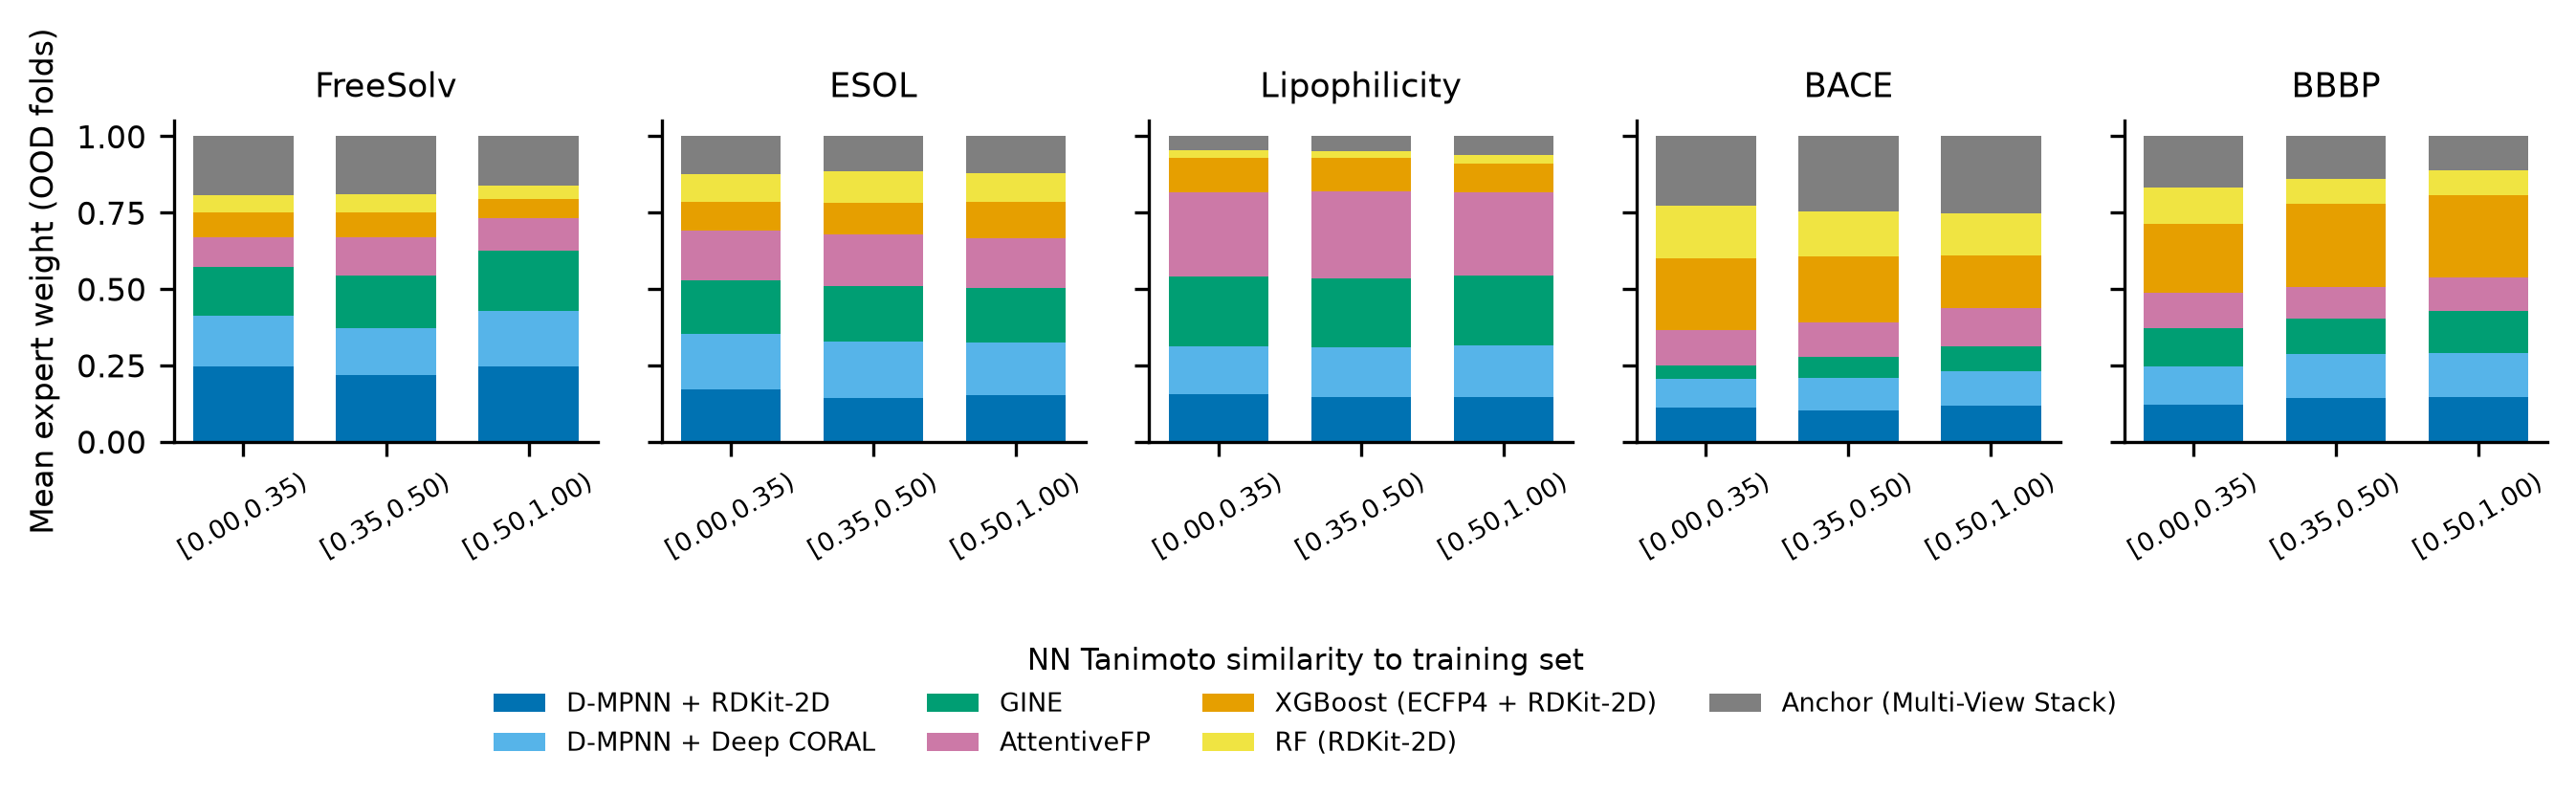
\includegraphics[width=\textwidth]{fig4_expert_weights.png}
\caption{Mean SIG-Net expert weights on OOD folds by dataset and novelty bin.}
\label{fig:weights}
\end{figure}

\subsection{Pre-registered confirmation on fresh splits}
To test whether the local components generalise beyond the splits on which they were developed, we generated four new seeds for every dataset and protocol with the same splitting code, cross-fitted nine experts (the seven above plus ChemBERTa-2 + XGBoost and XGBoost on ECFP4) and saved their out-of-fold, validation and test predictions, so that routers could be compared on identical expert outputs. Seed 11 was used for development; seeds 1--3 were not inspected until a refined router (SIG-Net v4, Methods) had been frozen and the primary endpoint registered (Supporting Information, Addendum 2). The \texttt{FreeSolv} generic-skeleton split yields the same test set for every seed and was excluded from the endpoint, leaving 57 folds (the plan erroneously stated 56).

The primary endpoint was met: SIG-Net v4 improved on the global stack of the seven original experts in 35/57 folds, mean +1.27\%, median +0.20\%, $p = 0.020$ (Table~\ref{tab:confirm}). The improvement is concentrated in the regression tasks---\texttt{FreeSolv} +7.4\%, \texttt{Lipophilicity} +0.6\% and \texttt{ESOL} +0.3\%---and absent on the classification tasks (\texttt{BACE} -0.1\%, \texttt{BBBP} -0.2\%; Figure~\ref{fig:confirm}). Of v4's components, only the local residual correction had a confirmed effect (v4 vs.\ v4 without it: 29/57 folds, mean +0.29\%, median +0.01\%, $p = 0.016$); the composite kernel ($p = 0.857$) and the novelty shrinkage ($p = 0.633$) did not. The local softmax weighting of the original router did not replicate: on the fresh folds it was indistinguishable from the global stack (28/57 folds, mean +0.27\%, median +0.00\%, $p = 0.805$), in contrast to its small advantage on the original seeds. The central result, by contrast, replicated strongly: SIG-Net v4 outperformed every individual cross-fitted expert, including D-MPNN+RDKit (48/57 folds, mean +5.10\%, median +2.43\%, $p = 7.3 \times 10^{-7}$) and ChemBERTa-2 + XGBoost (55/57 folds, mean +22.87\%, median +25.19\%, $p = 2.1 \times 10^{-10}$).

\begin{table}
\caption{Pre-registered confirmation on fresh seeds 1--3 (57 folds, \texttt{FreeSolv} generic skeleton excluded): SIG-Net v4 vs.\ each comparator. Relative improvement per fold (\%); two-sided Wilcoxon signed-rank test.}
\label{tab:confirm}
\scriptsize
\begin{tabular}{lcrrc}
\toprule
Comparator & Folds won & Mean (\%) & Median (\%) & $p$ \\
\midrule
Global stack (7 experts) & 35/57 & +1.27 & +0.20 & $p = 0.020$ \\
Global stack (9 experts) & 34/57 & +1.34 & +0.21 & $p = 0.019$ \\
Original router (local softmax, 7) & 34/57 & +0.91 & +0.19 & $p = 0.117$ \\
v4 w/o residual correction & 29/57 & +0.29 & +0.01 & $p = 0.016$ \\
v4 w/o composite kernel & 17/57 & +0.38 & +0.00 & $p = 0.857$ \\
v4 w/o novelty shrinkage & 22/57 & +0.02 & +0.00 & $p = 0.633$ \\
Multi-view anchor (bagged) & 42/57 & +6.18 & +3.06 & $p = 1.2 \times 10^{-5}$ \\
D-MPNN+RDKit (bagged) & 48/57 & +5.10 & +2.43 & $p = 7.3 \times 10^{-7}$ \\
AttentiveFP (bagged) & 47/57 & +5.09 & +2.67 & $p = 5.5 \times 10^{-7}$ \\
XGBoost ECFP4+RDKit (bagged) & 50/57 & +10.10 & +5.04 & $p = 2.1 \times 10^{-9}$ \\
ChemBERTa-2 + XGBoost (bagged) & 55/57 & +22.87 & +25.19 & $p = 2.1 \times 10^{-10}$ \\
\bottomrule
\end{tabular}
\end{table}

\begin{figure}
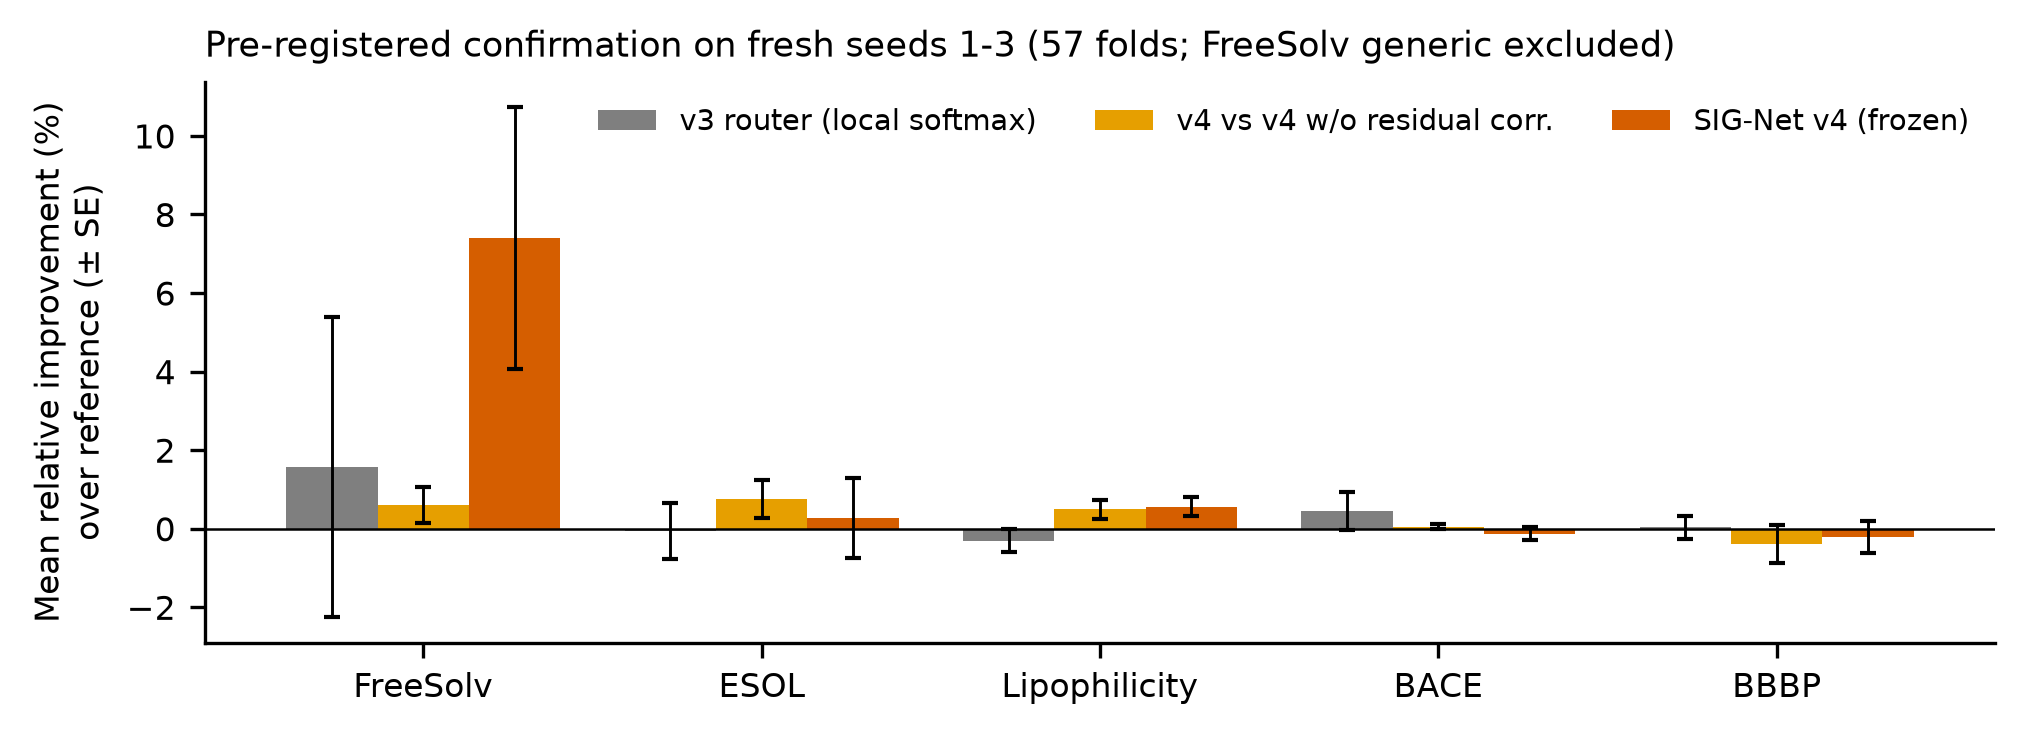
\includegraphics[width=\textwidth]{fig5_confirmatory.png}
\caption{Confirmation on fresh splits, by dataset (mean $\pm$ SE of per-fold relative improvement). Grey: original local-softmax router vs.\ global stack; red: SIG-Net v4 vs.\ global stack; orange: SIG-Net v4 vs.\ SIG-Net v4 without the residual correction.}
\label{fig:confirm}
\end{figure}

\section{Discussion}
Three practical conclusions follow. First, BM scaffold splits should not be read as tests of extrapolation to unseen ring systems: for most test molecules a closely related carbon skeleton is in the training set. Generic-skeleton splits are a simple alternative, but they can become degenerate on small datasets dominated by a few skeletons (here \texttt{FreeSolv}), which should be checked and reported. Second, because the best model varies across datasets and splits, combining diverse, cross-fitted experts is a more reliable default than selecting a single architecture; this is the part of SIG-Net that held up in every analysis, including the pre-registered confirmation on fresh splits. Third, the gains from making the combination local are small and endpoint-dependent. The original local softmax weighting looked significant on the discovery splits but did not replicate; a local out-of-fold residual correction did replicate, mainly on regression endpoints. The novelty-shrinkage exponent $\gamma$ had no measurable effect in any analysis, so we recommend omitting it: the simplest form of SIG-Net that retains its confirmed benefits is a global stack of cross-fitted diverse experts followed by a local out-of-fold residual correction whose strength $\nu$ and neighbourhood size $k$ are chosen on validation data.

\paragraph{Future work.}
The local error covariance used by SIG-Net v4 also yields a per-molecule error estimate, $\mathbf{w}(x)^\top\hat{\boldsymbol{\Sigma}}(x)\mathbf{w}(x)$, which could support locally adaptive conformal prediction intervals. Fine-tuned (rather than frozen) foundation models as experts, classification-specific local calibration, and evaluation on independent datasets such as ADMET panels and time splits\cite{sheridan2013timesplit} are the most direct next steps.

\paragraph{Limitations.}
The benchmark covers five MoleculeNet datasets of 642--4200 molecules, two of them classification tasks; larger, more diverse sets (e.g.\ ADMET panels or time splits\cite{sheridan2013timesplit}) remain to be tested. Hyperparameters of all models were fixed rather than tuned per dataset. The confirmation used three fresh seeds of the same five datasets, not independent datasets, and its mean gain is driven largely by \texttt{FreeSolv} (median gain +0.20\%). SIG-Net trains each expert five times per fold, roughly 20 times the cost of a single D-MPNN. A pretrained chemical language model (ChemBERTa-2) was evaluated only as a frozen-embedding baseline; fine-tuned foundation models, and their use as SIG-Net experts, remain to be tested. \texttt{BBBP} and the ChemBERTa-2 baselines were added after the pre-specified analysis and before their results were viewed (analysis-plan addendum, Supporting Information). The gain over the best global stack is small in absolute terms (median +0.14\%), and the Nemenyi test does not separate SIG-Net from the next-ranked models. Finally, in earlier versions of this pipeline, graph models received integer-coded atom features; with one-hot features (used throughout this work) the \texttt{FreeSolv} BM-scaffold RMSE of D-MPNN fell from 3.59 (integer features, five seeds) to 1.82, which illustrates how strongly featurisation choices affect comparisons between model families.

\section{Conclusions}
We quantified carbon-skeleton overlap under BM scaffold splits on five MoleculeNet benchmarks and introduced SIG-Net, a similarity-informed mixture of cross-fitted experts. Over 100 folds and 30 comparison models, SIG-Net achieved the best mean rank and outperformed every external model on paired comparisons. A pre-registered confirmation on fresh splits showed that this advantage comes from cross-fitted stacking of diverse experts, that a local out-of-fold residual correction adds a small further gain on regression endpoints, and that the original local weighting and the novelty-shrinkage term do not generalise.

\section{Data and Software Availability}
All datasets are public (MoleculeNet). The complete pipeline---curation, splitting, featurisation, all models, the 100-fold benchmark, statistics, figures and this manuscript---is provided as a single Jupyter notebook together with per-fold predictions and the pre-specified analysis plan. All code, the notebook, per-fold predictions, the analysis plan with its addenda and the frozen-design records are available at \url{https://github.com/bhaskargurram-ai/SIG-Net}; the curated data bundle with all split indices is attached to release v1.0 of that repository.

\begin{suppinfo}
Supporting Information: pre-specified analysis plan; full benchmark of all models (Table~S1); full rankings (Table~S2); all paired comparisons (Table~S3); per-setting results (Table~S4).
\end{suppinfo}





\bibliography{refs}
\end{document}
